%\section{Vélo cargo Douze G4e}
\section{Introduction}

\begin{center}
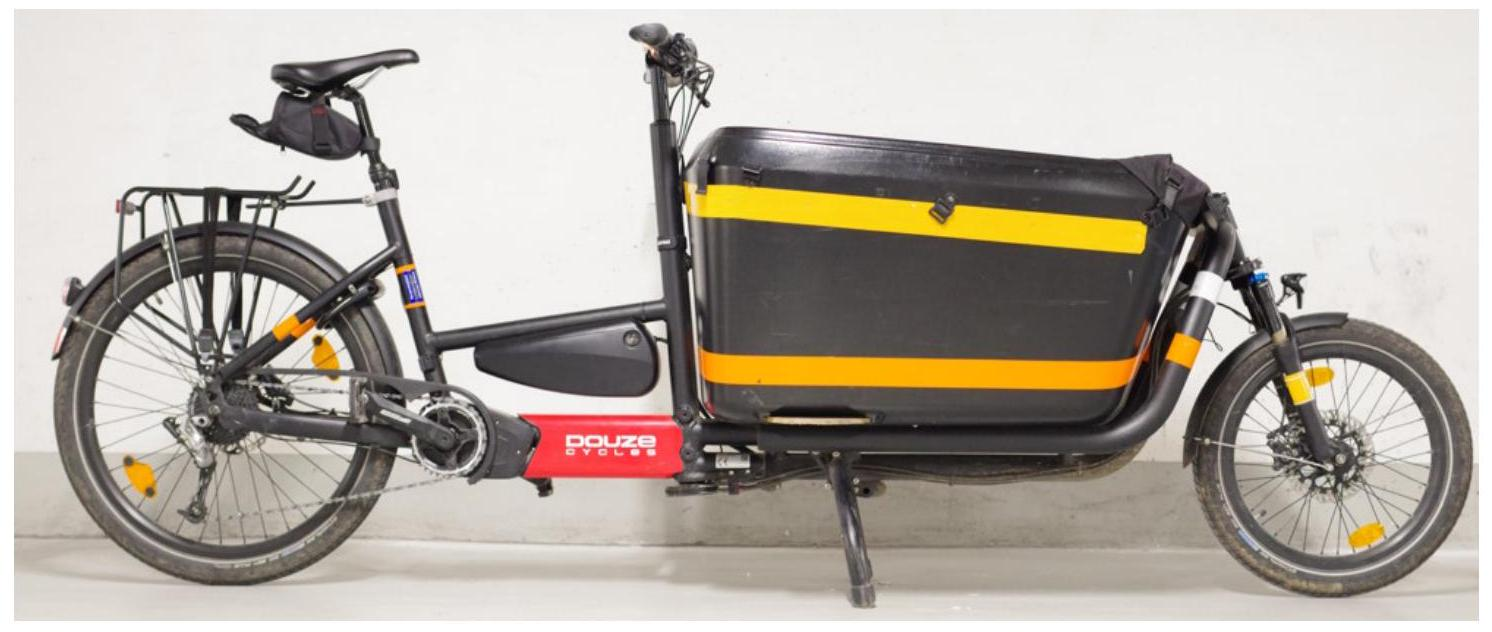
\includegraphics[width=0.8\textwidth]{2024_12_06_8b2ce2e701dae8972925g-01}
\end{center}


Le secteur des transports est la première source d'émissions de gaz à effet de serre en France avec \(31 \%\) des émissions du pays. Ces émissions sont, pour plus de moitié, dues aux véhicules individuels motorisés (voitures, motos) qui restent utilisés au quotidien par \(68 \%\) des Français alors que plus de la moitié des trajets effectués fait moins de \(5 \mathrm{~km}\)\footnote{Données extraites de l’article « Bouger autrement au quotidien » publié par l’ADEME  \url{https://librairie.ademe.fr/cadic/
7338/guide-bouger-autrement-au-quotidien.pdf}}.

À l'inverse, non content d'être un très faible émetteur de gaz à effet de serre, le vélo s'avère peu consommateur en ressources et en énergie tout en étant bon pour la santé individuelle et collective. Le vélo constitue également une solution viable pour décongestionner les villes. Son utilisation est encouragée par de nombreux acteurs institutionnels de par la création d'aménagements cyclables, les aides à l'achat de vélo à assistance électrique ou encore la création du forfait mobilité durable.

L'essor des vélos à assistance électrique (VAE) a libéré de nombreux cyclistes de l'appréhension du relief. Le développement des VAE s'est accompagné de celui des vélos cargos qui permettent d'effectuer des livraisons ou encore de transporter des enfants. Ce sujet porte sur un de ces vélos cargo.

\subsection{Présentation du système}

La société Douze cycles conçoit et réalise des vélos cargo destinés aux professionnels comme aux particuliers. Cette société est implantée en Bourgogne où elle emploie 25 collaborateurs.

Le système étudié est un biporteur à assistance électrique, le G4e, conçu et réalisé par Douze cycles. Soucieuse d'allier durabilité, praticité et esthétique, la société Douze cycles innove continument pour faire évoluer sa gamme de produits. Ce vélo, présenté par l'entreprise comme «~une solution vélogistique tout-en-un répondant à la plupart des usages pour les familles ou les professionnels~», a été lancé en 2017 pour le cinquième anniversaire de la marque.

\subsection{Étude proposée}
Les études proposées dans ce sujet portent sur différentes problématiques spécifiques à la conception du vélo cargo étudié.

\begin{itemize}
  \item L'étude s'ouvre, partie \ref{ATS_2024_sec2} sur la détermination de l'effort que doit fournir le cycliste pour garer le vélo sur sa béquille.
  \item La partie \ref{ATS_2024_sec3} aborde le dimensionnement des organes de freinage.
  \item La modélisation du capteur utilisé pour mesurer le couple appliqué par le cycliste sur le pédalier occupe la partie \ref{ATS_2024_sec4}.
  \item La partie \ref{ATS_2024_sec5} se focalise sur l'étude de l'association \{ onduleur + machine \} qui anime le groupe d'assistance.
  \item Enfin, les modèles obtenus lors des deux parties précédentes sont exploités partie \ref{ATS_2024_sec6} lors de l'étude de l'asservissement du couple délivré par la machine du groupe d'assistance.\\
Les différentes parties de cette étude sont indépendantes.
\end{itemize}

%\footnotetext{\begin{enumerate}
%  \item Données extraites de l'article « Bouger autrement au quotidien » publié par l'ADEME \href{https://librairie.ademe.fr/cadic/}{https://librairie.ademe.fr/cadic/} 7338/guide-bouger-autrement-au-quotidien.pdf
%\end{enumerate}
%}

\section{Effort de mise en stationnement \label{ATS_2024_sec2}}

\begin{obj}
Déterminer l'effort à exercer par l'usager lors de la mise en stationnement sur béquille.
\end{obj}

La mise en position parking du vélo cargo (le « béquillage») nécessite d'exercer un effort sur le guidon. Cette partie vise à déterminer cet effort et à vérifier sa compatibilité avec les exigences d'ergonomie.\\

\begin{figure}[!htb]
\begin{center}
%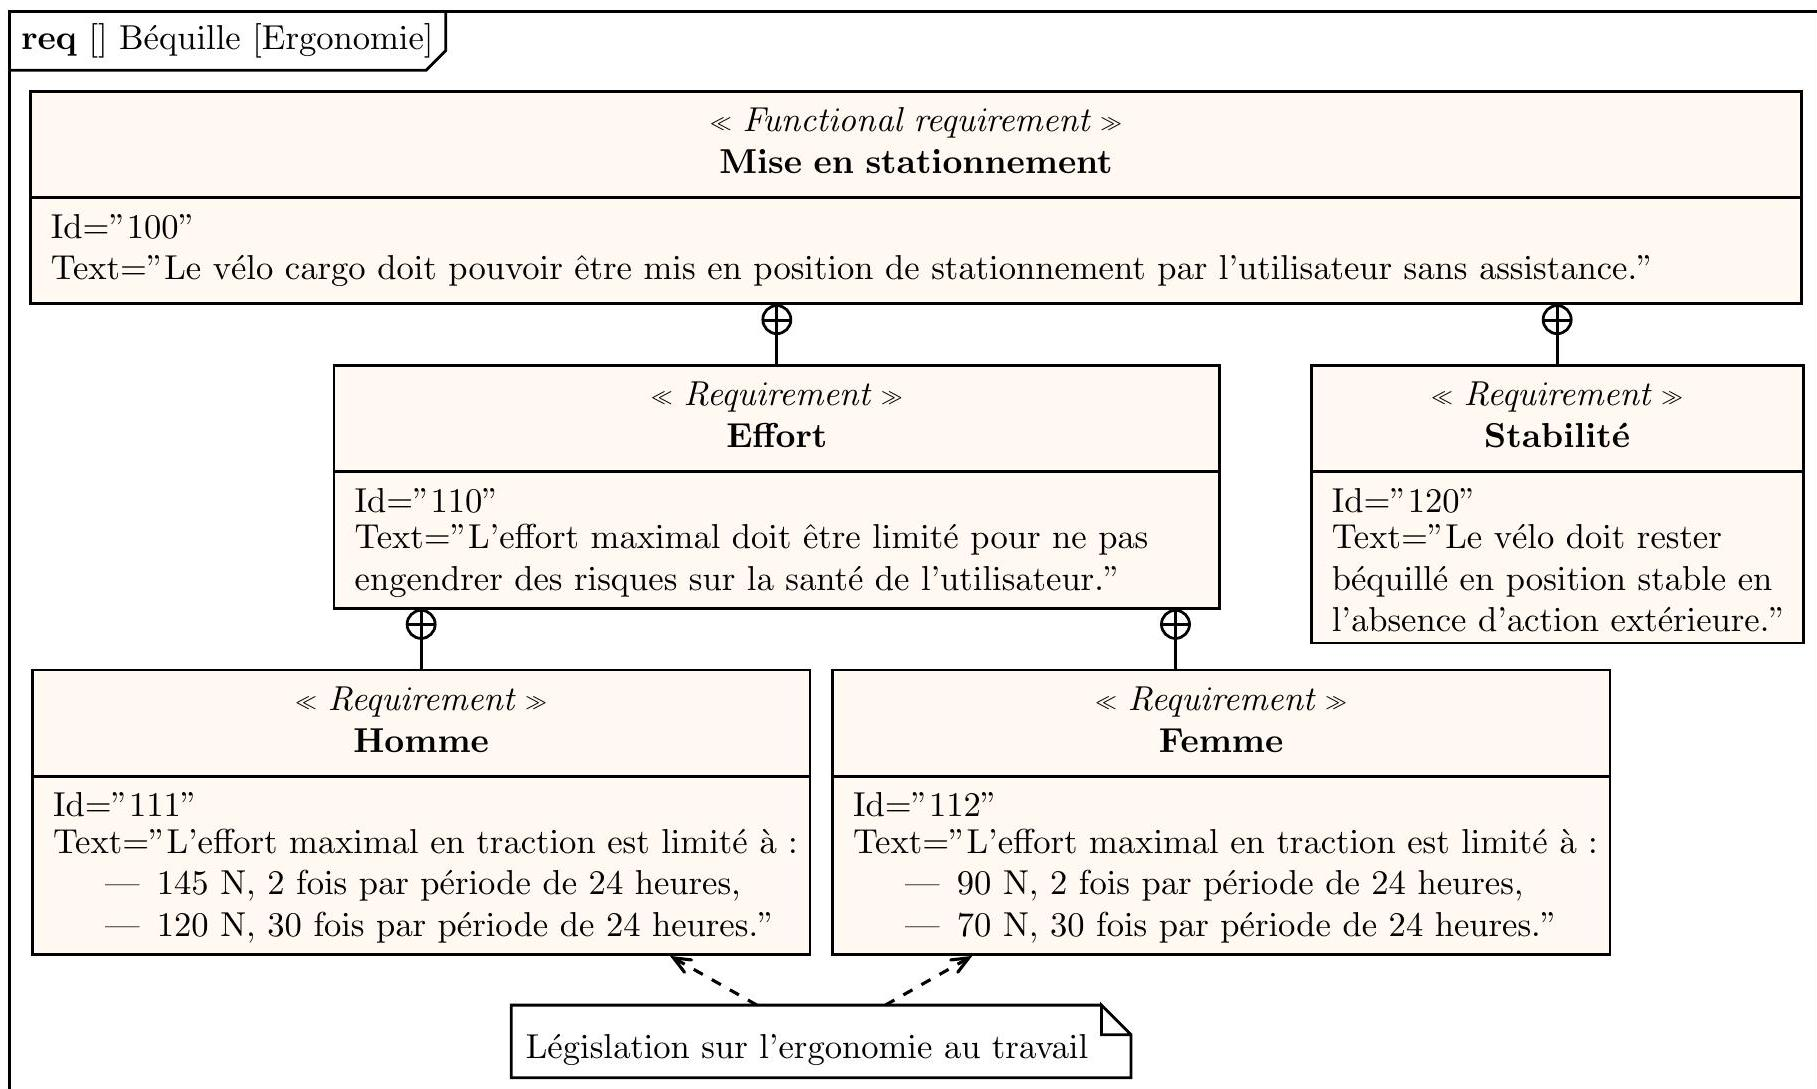
\includegraphics[width=.8\linewidth]{2024_12_06_8b2ce2e701dae8972925g-02}
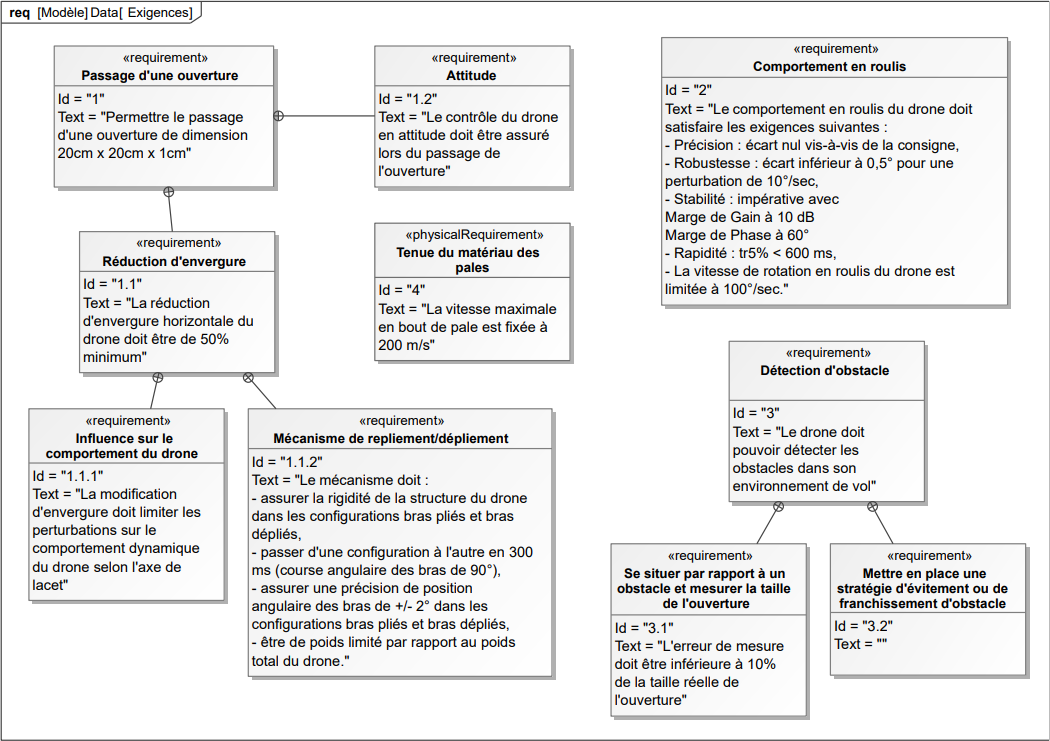
\includegraphics[width=.9\linewidth]{fig_21}
\caption{Extrait du cahier des charges relatif à l'ergonomie de la mise en stationnement du vélo\\ \label{fig2.1}}
\end{center}
\end{figure}

\begin{figure}[!htb]
\begin{center}
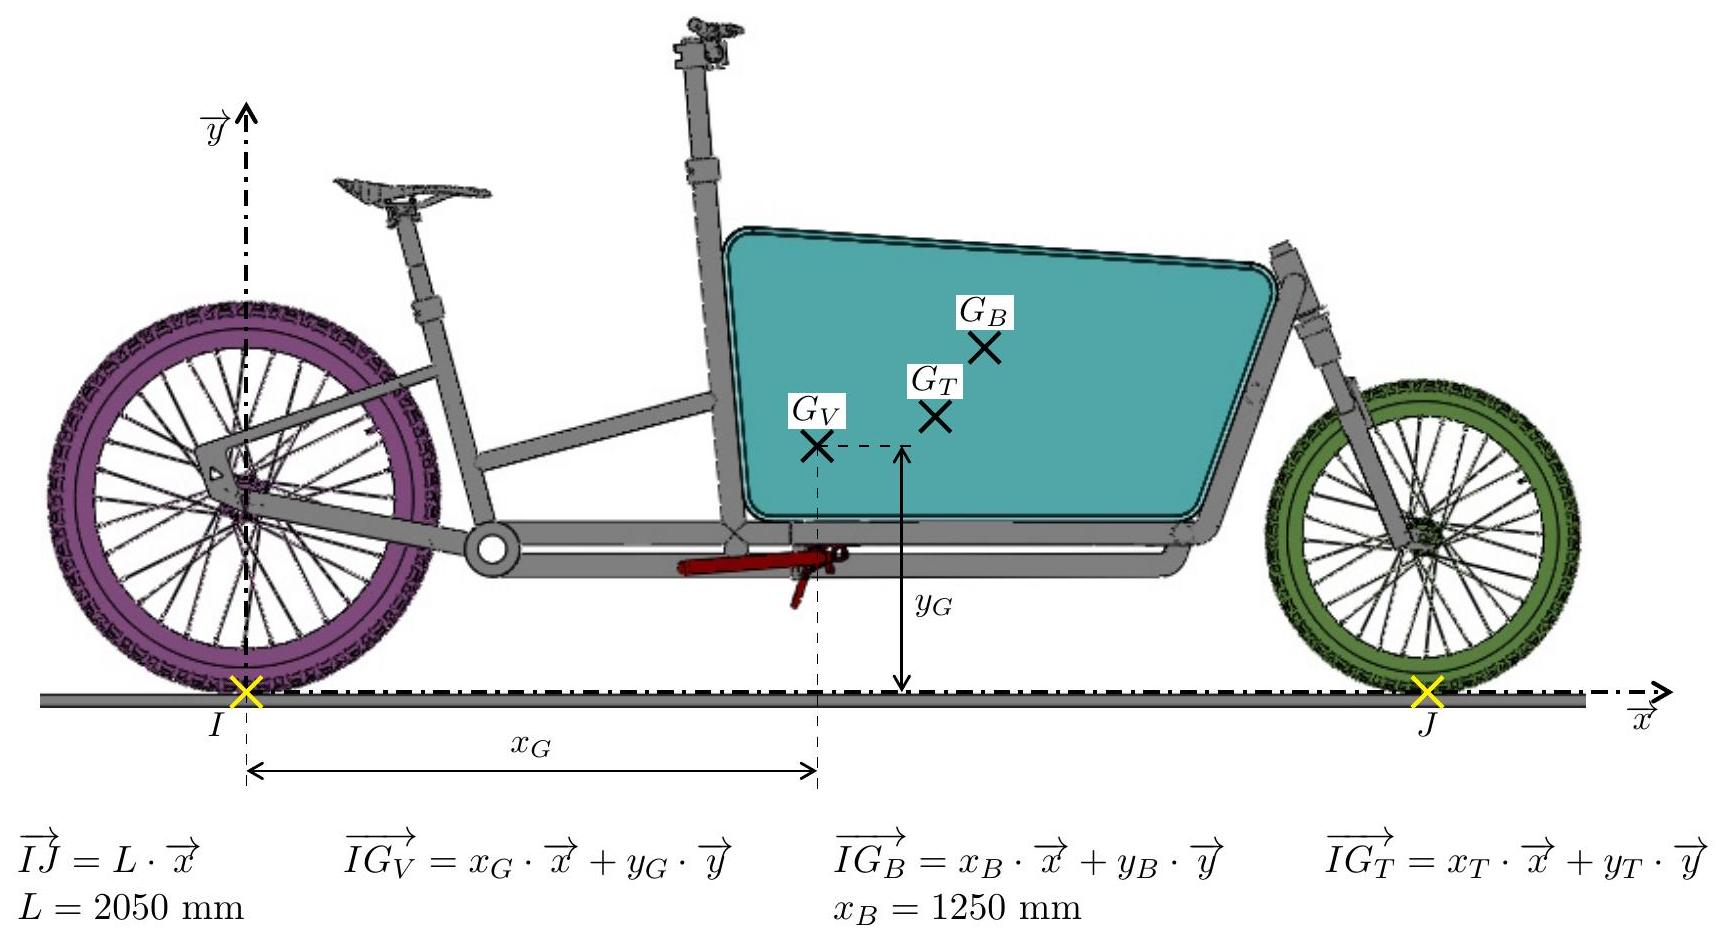
\includegraphics[width=0.8\textwidth]{2024_12_06_8b2ce2e701dae8972925g-02(1)}
\caption{Paramétrage adopté pour la détermination des caractéristiques inertielles du vélo \label{fig2.2}}
\end{center}
\end{figure}


\subsection{Caractéristiques inertielles du vélo}
\paragraph*{Définition des ensembles}
\begin{itemize}
  \item \(V\) : ensemble du vélo hors béquille (supposée de masse négligeable) et hors black-box;
  \item \(B\) : black-box chargée au maximum;
  \item \(T=V \cup B\).
\end{itemize}

\subsubsection{Centre de gravité \(G_{V}\) du vélo à vide}
On étudie le vélo G4e à vide (ensemble \(V\) ). La masse totale de cet ensemble est alors \(m_{V}=49 \mathrm{~kg}\). Les roues du vélo ainsi équipé sont positionnées sur des balances, l'ensemble étant en équilibre dans le plan vertical \((I ; \vec{x}, \vec{y})\). On mesure au niveau des points de contact:
\begin{itemize}
\item arrière, \(I: m_{I}=26 \mathrm{~kg}\);
  \item avant, \(J: m_{J}=23 \mathrm{~kg}\).
\end{itemize}
La distance entre les points \(I\) et \(J\) est notée \(L=2050 \mathrm{~mm}\) (voir figure \ref{fig2.2}).\\


\question{Déterminer l'expression littérale de la position \(x_{G}\) suivant \(\vec{x}\) du centre de gravité de l'ensemble. En déduire la valeur de \(x_{G}\) en mm (on arrondira le résultat à la dizaine de mm ).}
\ifprof
\begin{corrige}-- [UPSTI]
On isole le vélo. En utilisant le Principe Fondamental de la Statique (PFS) en moment au point $I$ sur $\vect{z}$, on obtient :
$-m_V x_G+m_J L=0$ 
$\Rightarrow m_V x_G = m_J L$
$\Rightarrow x_G=\dfrac{m_J}{m_V}  L=\dfrac{m_J}{m_I+m_J}  L$

A.N. $x_G=\dfrac{23}{26+23}2050$ $\Rightarrow  x_G \simeq \SI{960}{mm}$.

\end{corrige}
\else
\fi

\subsubsection{Centre de gravité \(G_{T}\) du vélo chargé}
On considère à présent que la black box est chargée à son maximum ( \(m_{B}=100 \mathrm{~kg}\) ). On appelle \(G_{B}\), le centre de gravité de la masse chargée où \(x_{B}=1250 \mathrm{~mm}\)

\question{Déterminer l'expression littérale de la position \(x_{T}\) suivant \(\vec{x}\) du centre de gravité de l'ensemble chargé. Calculer la valeur, arrondie à la dizaine de mm , de \(x_{T}\).}
\ifprof
\begin{corrige}-- [UPSTI]
En utilisant la formule du barycentre, on obtient :
$(m_B+m_V ) \vect{OG_T}  =m_B \vect{OG_B}+m_V \vect{OG_V}$ $\Rightarrow  (m_B+m_V ) x_T=m_B x_B+m_V x_G$ $\Leftrightarrow  x_T=\dfrac{m_B x_B+m_V x_G}{m_B+m_V}$.

A.N. $x_T=\dfrac{100\times 1250+49\times 960}{100+49} \Leftrightarrow x_T=\SI{1150}{mm}$.

\end{corrige}
\else
\fi

\subsection{Étude géométrique}
L'étude est menée dans le plan \((I ; \vec{x}, \vec{y})\) à partir du paramétrage défini figure \ref{fig_23}.

\paragraph*{Procédure de béquillage} Le béquillage se réalise en poussant la béquille avec le pied sur le sol puis en exerçant une action de traction sur le guidon.

L'utilisateur garde son pied sur la béquille pour la plaquer au sol durant toute la phase de béquillage afin de maintenir le contact en \(K\) de la béquille avec le sol.

\paragraph*{Mouvement du vélo} On suppose dans cette partie que la fourche avant est rigide durant la phase de béquillage. Dès lors, la roue avant se décollera du sol sous l'action de traction du vélo par l'usager tandis que la roue arrière reculera.

\paragraph*{Définition de l'ensemble étudié :} L'ensemble étudié se compose des solides suivants :
\begin{itemize}
  \item le sol (0), repère associé ( \(I ; \vec{x}, \vec{y}, \vec{z})\);
  \item la roue arrière (1);
  \item le cadre (2), repère associé \(\left(A ; \overrightarrow{x_{c}}, \overrightarrow{y_{c}}, \vec{z}\right)\);
  \item la béquille (4), repère associé \(\left(A ; \overrightarrow{x_{b}}, \overrightarrow{y_{b}}, \vec{z}\right)\);
  \item la roue avant (3).
\end{itemize}


\paragraph*{Modèle cinématique} On modélise la cinématique de l'ensemble par une liaison :

\begin{itemize}
  \item sphère/plan en \(I\) suivant \(\vec{y}\) entre la roue arrière (1) et le sol (0);
  \item pivot d'axe \(( B ; \vec{z})\)  entre la roue (1) et le cadre (2);
  \item pivot d'axe \((A ; \vec{z})\) entre le cadre (2) et la béquille (4);
  \item pivot d'axe \((K ; \vec{z})\) entre la béquille (4) et le sol (0) (modélisation associée au blocage de la béquille par le pied).
\end{itemize}

\begin{figure}[!htb]
\centering

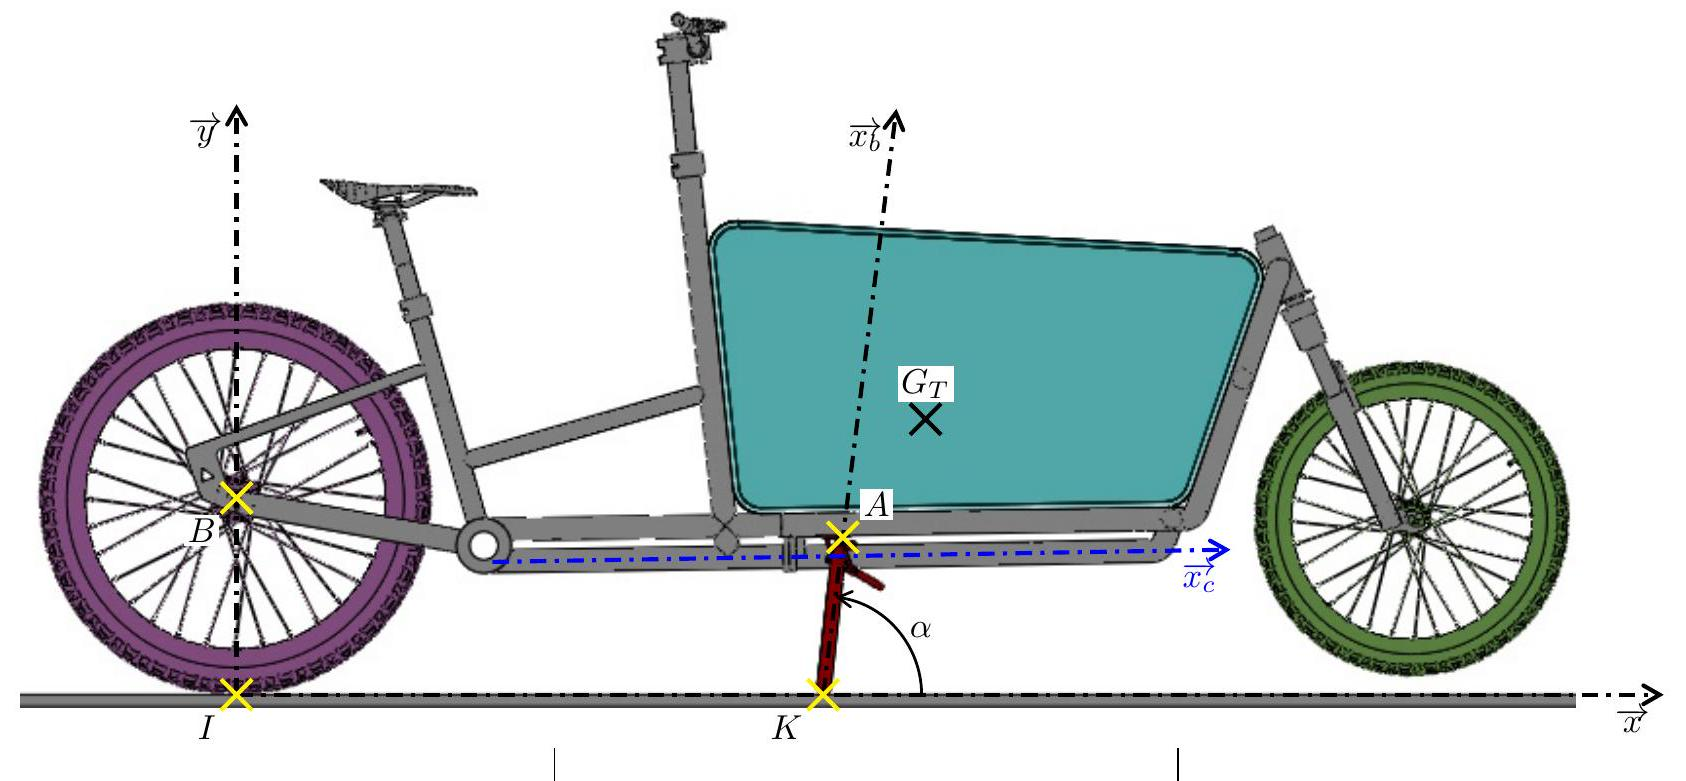
\includegraphics[width=0.8\textwidth]{2024_12_06_8b2ce2e701dae8972925g-04(1)}

\begin{tabular}{p{5cm}p{5cm}p{5cm}}
$
\begin{aligned}
\overrightarrow{K I} & =\mu(t) \cdot \vec{x} \\
\overrightarrow{K A} & =a \cdot \overrightarrow{x_{b}} \\
\overrightarrow{I B} & =R_{B} \cdot \vec{y} \\
\overrightarrow{A B} & =-b \cdot \overrightarrow{x_{c}}+e \cdot \overrightarrow{y_{c}} \\
\overrightarrow{A G_{T}} & =\left(x_{T}-b\right) \cdot \overrightarrow{x_{c}}+\left(y_{T}-h\right) \cdot \overrightarrow{y_{c}}
\end{aligned}
$
&
$
\begin{aligned}
a & =290 \mathrm{~mm} \\
R_{B} & =340 \mathrm{~mm} \\
b & =1030 \mathrm{~mm} \\
e & =70 \mathrm{~mm} \\
h & =270 \mathrm{~mm} \\
x_{T} & =1150 \mathrm{~mm} \\
y_{T} & =400 \mathrm{~mm}
\end{aligned}
$
&
$
\begin{aligned}
& \alpha(t)=\left(\vec{x}, \overrightarrow{x_{b}}\right)=\left(\vec{y}, \overrightarrow{y_{b}}\right) \\
& \beta(t)=\left(\vec{x}, \overrightarrow{x_{c}}\right)=\left(\vec{y}, \overrightarrow{y_{c}}\right)
\end{aligned}
$
La partie basse du cadre est à l'horizontale avant le béquillage : \(\overrightarrow{x_{c}}\) et \(\vec{x}\) sont colinéaires lorsque les deux roues sont en contact avec le sol.
\\
\end{tabular}
% FIG 2.3
\caption{\label{fig_23} Paramétrage utilisé pour l'étude du béquillage}

\end{figure}



\question{Recopier et compléter le schéma cinématique esquissé ci-dessous, conformément au modèle, proposé en faisant apparaître les liaisons, les solides et les repères qui leurs sont associés.}
\ifprof
\begin{corrige}-- [UPSTI]
\end{corrige}
\else
\fi
\begin{center}
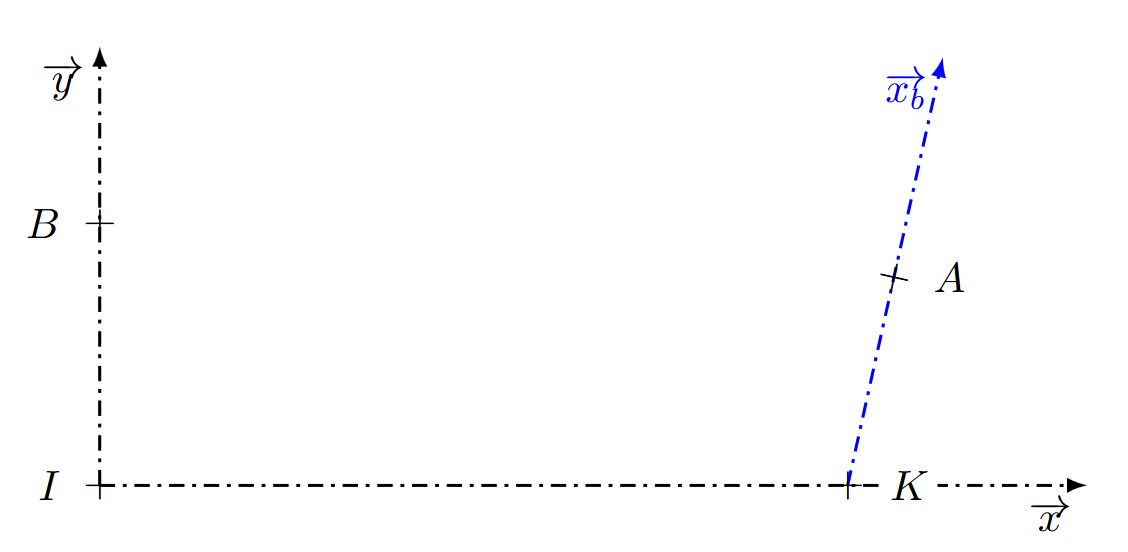
\includegraphics[width=.7\linewidth]{dr_q3}

Schéma à recopier et compléter
\end{center}

\question{Recopier et compléter les figures de calcul esquissées ci-dessous.}
\ifprof
\begin{corrige}-- [UPSTI]
\end{corrige}
\else
\fi

\begin{center}
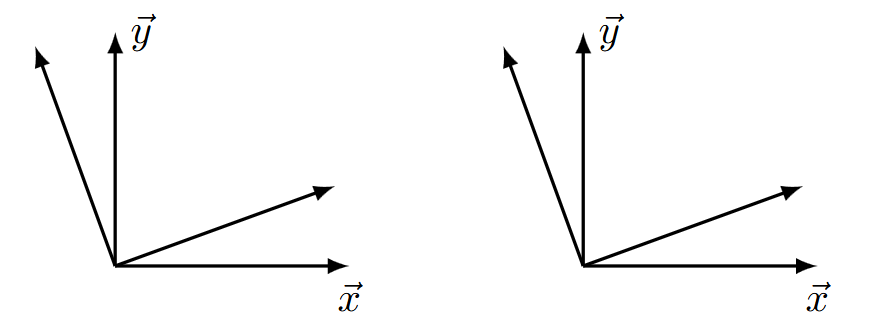
\includegraphics[width=.7\linewidth]{dr_q4}
\end{center}

\question{À partir d'une fermeture géométrique, montrer que l'équation scalaire qui lie la valeur de \(\beta\) à \(\alpha, a, b, e\) et \(R_{B}\) est de la forme : \(a \cdot \sin (\alpha)=b \cdot \sin (\beta)-e \cdot \cos (\beta)+R_{B}\).}
\ifprof
\begin{corrige}-- [UPSTI]
La fermeture géométrique $\vect{IK}+\vect{KA}+\vect{AB}+\vect{BI}=\vect{0}$ donne l’équation vectorielle :
$-\mu\vect{x}+a\vect{x_b}-b\vect{x_c}+e\vect{y_c}-R_B \vect{y} = \vect{0}$.
La projection sur  $\vect{y}$ de cette relation permet d’obtenir $a\sin\alpha -b\sin\beta +e\cos\beta-R_B=0$.
$\Rightarrow  a\sin\alpha =b\sin\beta -e\cos\beta +R_B$.

\end{corrige}
\else
\fi

\paragraph*{Valeurs limites de \(\alpha\)} On note \(\alpha_{i}\) et \(\alpha_{f}\left(\alpha_{i}<\alpha_{f}\right)\) les valeurs de l'angle \(\alpha\) entre lesquelles la roue avant est décollée du sol.

\question{Déterminer les expressions des angles \(\alpha_{i}\) et \(\alpha_{f}\) en fonction de \(R_{B}\), e et \(a\). En calculer les valeurs en radians.}
\ifprof
\begin{corrige}-- [UPSTI]
Au cours du mouvement, l’angle $\beta$ reste faible, on peut donc utiliser les approximations $\cos\beta\simeq 1$ et $\sin\beta\simeq 0$.
Ainsi $\sin\alpha=\dfrac{R_B-e}{a} \Rightarrow \left\{ \begin{array}{l} 
\alpha_i=\arcsin\dfrac{R_B-e}{a} \\
\alpha_f=\pi -\arcsin \dfrac{R_B-e}{a}
\end{array}\right.$

A.N. $\alpha_i=66,8\degres$ et $\alpha_f=111,4\degres$ (ce qui correspond aux valeurs données dans la suite du sujet).

\end{corrige}
\else
\fi

Les valeurs calculées précédemment arrondies conduisent à \(\alpha_{i} \approx 70^{\circ}\) et \(\alpha_{f} \approx 110^{\circ}\). L'évolution de l'angle \(\beta\) en fonction de \(\alpha\), pour la plage de béquillage, est donnée figure \ref{fig_24}.

\question{Déduire de la courbe fournie la valeur d'inclinaison maximale du cadre par rapport au sol, notée \(\beta_{\max }\). Conclure sur l'hypothèse d'étude suivante : «Le cadre sera supposé horizontal lors du béquillage ».}
\ifprof
\begin{corrige}-- [UPSTI]
D’après la figure \ref{fig_24}, $\indice{\beta}{max}=1,1\degres$. Cet angle est très faible et permet bien de valider l’hypothèse stipulant que le cadre est supposé horizontal lors du béquillage.
\end{corrige}
\else
\fi

\begin{figure}[!htb]
\begin{center}
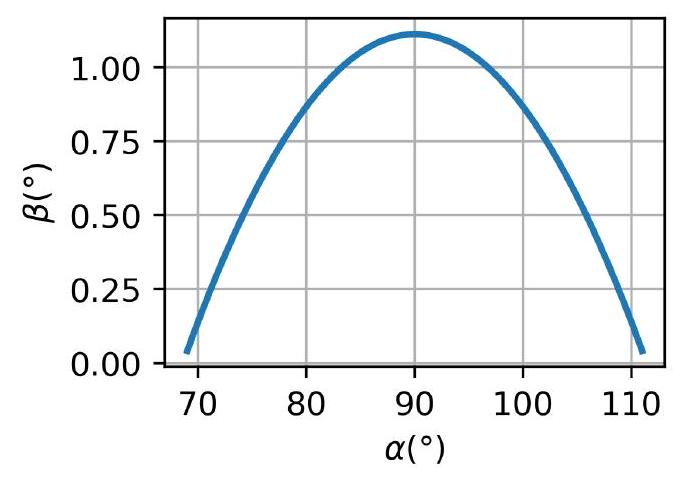
\includegraphics[width=.4\linewidth]{2024_12_06_8b2ce2e701dae8972925g-04}
\caption{Évolution de \(\beta\) en fonction de \(\alpha\) au cours du béquillage. \label{fig_24}}
\end{center}
\end{figure}


\subsection{Effort de béquillage}
On se propose à présent d'estimer l'action mécanique que doit développer le cycliste sur le guidon lors du béquillage dans le cas où la béquille est perpendiculaire au cadre (\(\alpha=90^{\circ}\), on admet qu'il s'agit de la position critique en termes d'effort). Le paramétrage adopté pour cette étude est défini figure \ref{fig_25}.\\

\begin{figure}[!htb]
\begin{center}
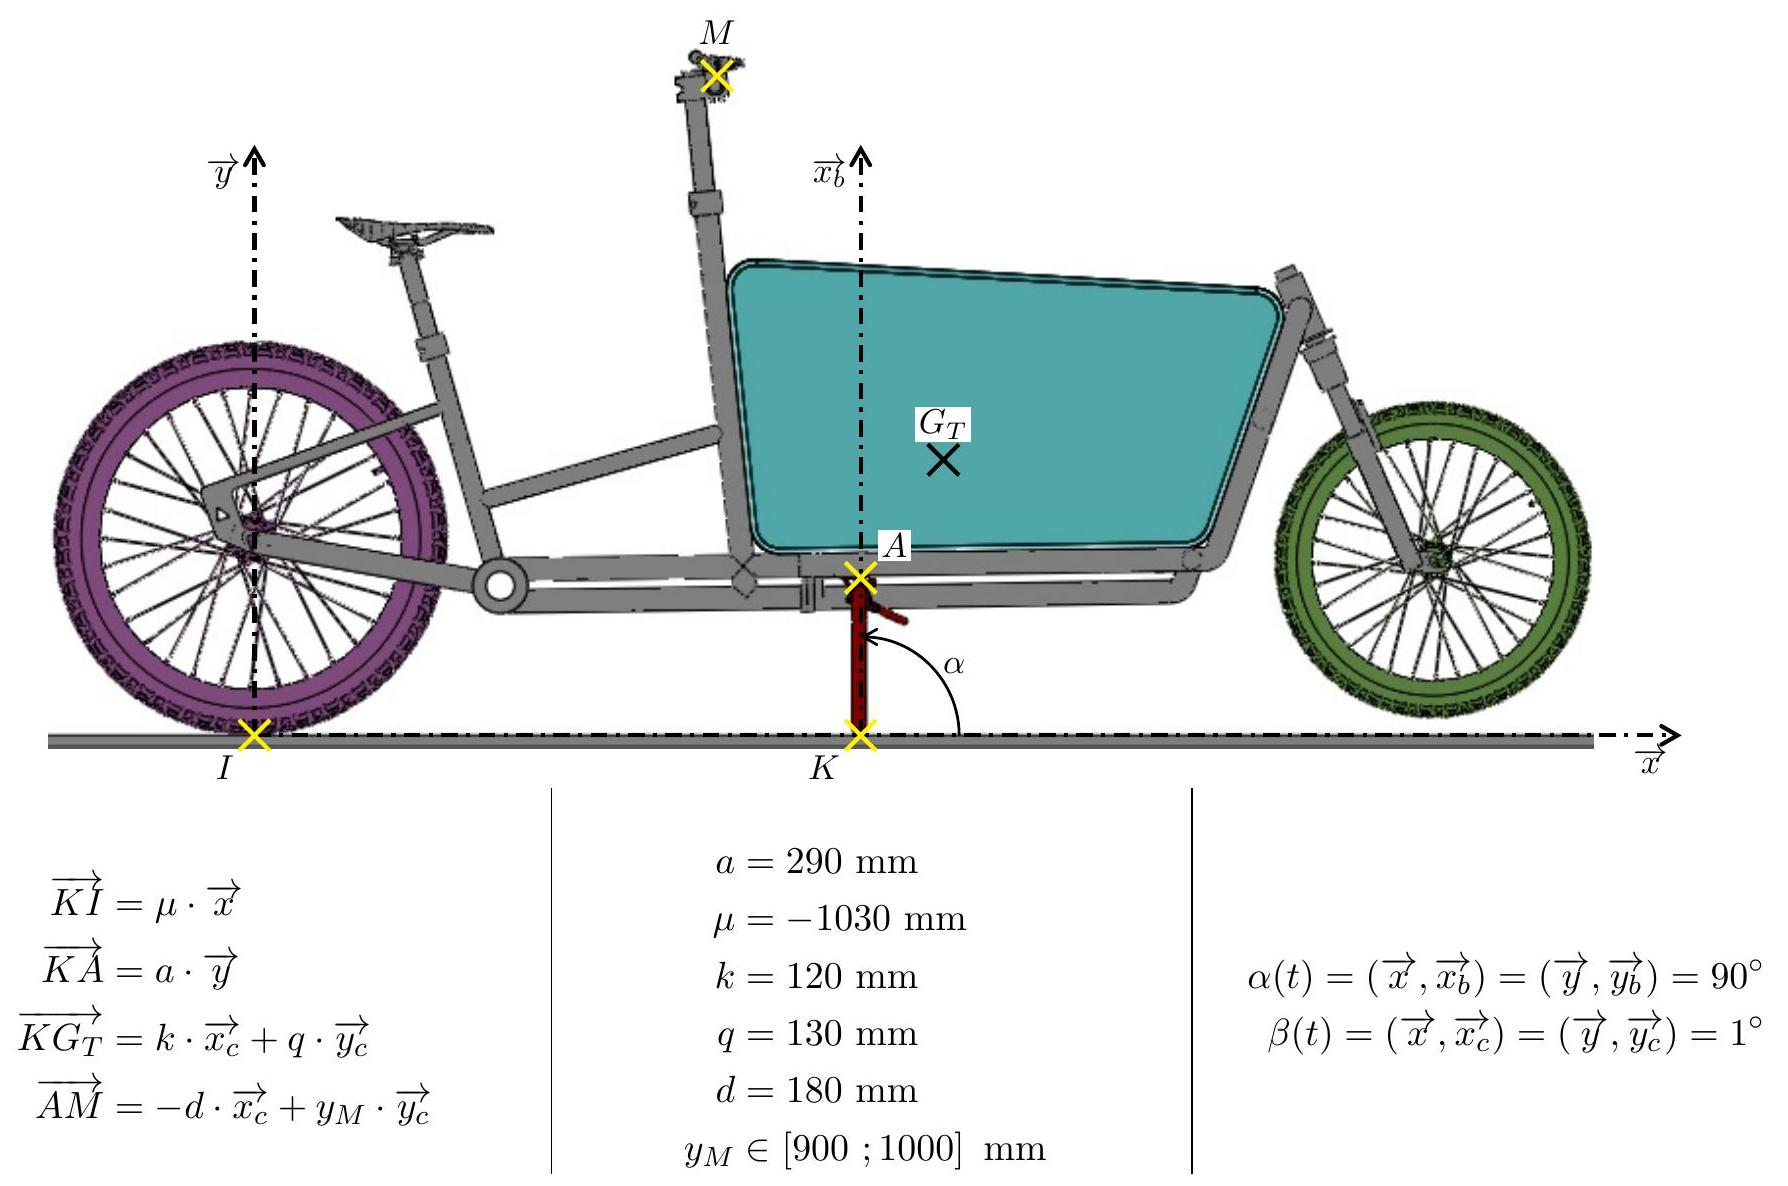
\includegraphics[width=0.8\textwidth]{2024_12_06_8b2ce2e701dae8972925g-05}
\caption{Paramétrage utilisé pour la détermination de l'effort à appliquer sur le guidon \label{fig_25}}
\end{center}
\end{figure}


Notation Le torseur de l'action mécanique exercée par le solide \(i\) sur \(j\), dans la base ( \(\vec{x}, \vec{y}, \vec{z}\) ), dans l'hypothèse de problème plan, est noté :
$
\{i \rightarrow j\}=\left\{\begin{array}{c|c}
X_{i j} & - \\
Y_{i j} & - \\
- & N_{i j}^{K}
\end{array}\right\}_{(\vec{x}, \vec{y}, \vec{z})} \quad \text { ou } \quad\{i \rightarrow j\}=_{K}\left\{\begin{array}{c}
X_{i j} \cdot \vec{x}+Y_{i j} \cdot \vec{y} \\
N_{i j}^{K} \cdot \vec{z}
\end{array}\right\}
$

\paragraph*{Données et hypothèses}
\begin{itemize}
  \item L'action mécanique exercée par le cycliste est un glisseur \(\overrightarrow{F_{C}}\) appliqué en \(M\) tel que \(\overrightarrow{F_{C}}=-F_{C} \cdot \vec{x}\).
  \item L'accélération de la pesanteur vaut \(\vec{g}=-g \cdot \vec{y}\) où on approche \(g\) par \(g=10 \mathrm{~m} / \mathrm{s}^{2}\).
  \item La masse de l'ensemble, pour rappel, est notée \(m_{T}\) et vaut \(m_{T}=149 \mathrm{~kg}\).
  \item On suppose les liaisons sans frottements à l'exception du contact Roue/Sol, où l'on suppose un frottement suivant le modèle de Coulomb de coefficient \(f=1\).
\end{itemize}

\question{Donner la forme du torseur des actions mécaniques transmissibles du sol ( 0 ) sur la béquille (4) en \(K\) dans la base ( \(\vec{x}, \vec{y}, \vec{z})\).}
\ifprof
\begin{corrige}-- [UPSTI]
$\{0 \rightarrow 4\}=\left\{\begin{array}{c}
X_{04} \cdot \vec{x}+Y_{04} \cdot \vec{y} \\
\vec{0}
\end{array}\right\}_{K}
$
\end{corrige}
\else
\fi

\question{Donner la forme du torseur des actions mécaniques transmissibles du sol (0) sur la roue (1) en \(I\) dans la base \((\vec{x}, \vec{y}, \vec{z})\).}
\ifprof
\begin{corrige}-- [UPSTI]
$\{0 \rightarrow 1\}=\left\{\begin{array}{c}
X_{01} \cdot \vec{x}+Y_{01} \cdot \vec{y} \\
\vec{0}
\end{array}\right\}_{I}
$
\end{corrige}
\else
\fi

\question{Donner la forme du torseur des actions mécaniques exercées par la pesanteur sur l'ensemble \(\Sigma=\{1,2,3,4\}\) en \(G_{T}\) dans la base ( \(\vec{x}, \vec{y}, \vec{z}\) ).}
\ifprof
\begin{corrige}-- [UPSTI]
$\{\text{pes} \rightarrow \Sigma \}=\left\{\begin{array}{c}
-m_T g\vect{y}  \\
\vec{0}
\end{array}\right\}_{G_T}
$

\end{corrige}
\else
\fi

\question{Appliquer le théorème du moment statique à \(\Sigma\) en \(I\) en projection sur \(\vec{z}\). En déduire la relation qui lie \(F_{C}\) à \(Y_{04}\) en fonction de \(\mu, a, k, q, d, y_{M}, \beta, m_{T}\) et \(g\).}
\ifprof
\begin{corrige}-- [UPSTI]
On isole le système ${\Sigma}$.
BAME :
\begin{itemize}
\item $\torseurstat{T}{0}{4}$
\item $\torseurstat{T}{\text{pes}}{\Sigma}$
\item $\torseurstat{T}{0}{1}$
\item $\torseurstat{T}{\text{cy}}{4}$
\end{itemize}

On calcule tous les moments au point I en utilisant la formule de Varignon.
$\vectm{I}{\text{Pes}}{\Sigma} $
$= \vectm{G_T}{\text{Pes}}{\Sigma} + \vect{IG_T}\wedge \left(-m_T g\vect{y}\right)$
$=\left(\vect{IK}+\vect{KG}\right) \wedge \left(-m_T g\vect{y}\right)$
$ = \left(-\mu \vect{x} + k\vect{x_c}+q\vect{y_c}\right) \wedge \left(-m_T g\vect{y}\right)$
$\left(\mu -k\cos\beta+q\sin\beta \right) m_T g\vect{z}$

$\vectm{I}{0}{4} = -\mu \vect{x} \wedge \left(X_{04}\vect{x}+Y_{04}\vect{y}\right) =-\mu Y_{04}\vect{z}$

$\vectm{I}{Cy}{4} =\left(\mu \vect{x} + a\vect{y} - d\vect{x_c} +y_M \vect{y_c}\right) \wedge -F_C\vect{x}$
$=(a-d\sin\beta +y_M \cos\beta) F_C = 0$.
On applique le PFS en moment au point $I$ sur $\vect{z}$ : 
$\left(\mu -k\cos\beta+q\sin\beta \right) m_T g - \mu Y_{04}+\left(a-d\sin\beta +y_M \cos\beta\right) F_C = 0$.

Ainsi, $F_C=\dfrac{\mu Y_{04}-(\mu -k\cos\beta +q\sin\beta) m_T g}{a-d\sin\beta+y_M \cos\beta}$.

\end{corrige}
\else
\fi

On suppose que \(\beta\) est suffisamment petit pour considérer que \(\sin \beta \approx 0\) et \(\cos \beta \approx 1\).\\



\question{Montrer qu'alors, on peut exprimer \(F_{C}\) sous la forme :
$F_{C} \approx \dfrac{\mu \cdot Y_{04}-(\mu-k) \cdot m_{T} \cdot g}{y_{M}+a}$.
Déterminer la condition sur \(y_{M}\) qui conduit alors à une action à développer par le cycliste \(F_{C}\) maximale.}
\ifprof
\begin{corrige}-- [UPSTI]
\end{corrige}
\else
\fi

\question{En isolant l'ensemble \(\Sigma\) et en appliquant le théorème de la résultante statique, écrire les équations scalaires qui relient les différentes composantes des torseurs d'actions mécaniques exercées par le sol.}
\ifprof
\begin{corrige}-- [UPSTI]
\end{corrige}
\else
\fi

\question{Montrer alors, que même en supposant le glissement en \(I\), l'isolement de l'ensemble ne permet pas de déterminer l'action du cycliste.}
\ifprof
\begin{corrige}-- [UPSTI]
\end{corrige}
\else
\fi

On se propose à présent d'isoler la béquille (4) seule. On fait l'hypothèse que son poids est négligeable devant les autres actions mécaniques.

\question{Montrer en appliquant le PFS à la béquille (4) et en choisissant une équation scalaire pertinente parmi celles disponibles, que pour la position étudiée (\(\alpha=90^{\circ}\)) et pour l'isolement choisi, \(X_{04}=0\) \footnote{$X_{03}$ dans le sujet initial.}.}
\ifprof
\begin{corrige}-- [UPSTI]
\end{corrige}
\else
\fi

On montre alors en utilisant les résultats précédents :
$F_{C}=\dfrac{f \cdot k \cdot m_{T} \cdot g}{\mu+f \cdot\left(y_{M}+a\right)}$.

On estime alors l'effort minimal pour assurer le béquillage en charge maximale à \(F_{C} \approx 80 \mathrm{~N}\).

\question{Conclure sur le respect de l'exigence 110 du cahier des charges du vélo (figure \ref{fig2.1}).}
\ifprof
\begin{corrige}-- [UPSTI]
\end{corrige}
\else
\fi

\section{Vérification du dimensionnement des organes participant au freinage \label{ATS_2024_sec3}}
La sécurité des utilisateurs du vélo cargo passe par un freinage performant. Les pneumatiques et les freins doivent garantir une distance d'arrêt du vélo raisonnable même lorsque celui-ci est chargé au maximum. L'étude proposée dans cette partie vise à vérifier le dimensionnement de ces éléments à la lumière du cahier des charges précisé dans le diagramme des exigences de la figure \ref{fig_3_cargo}.

\begin{figure}[!h]
\centering
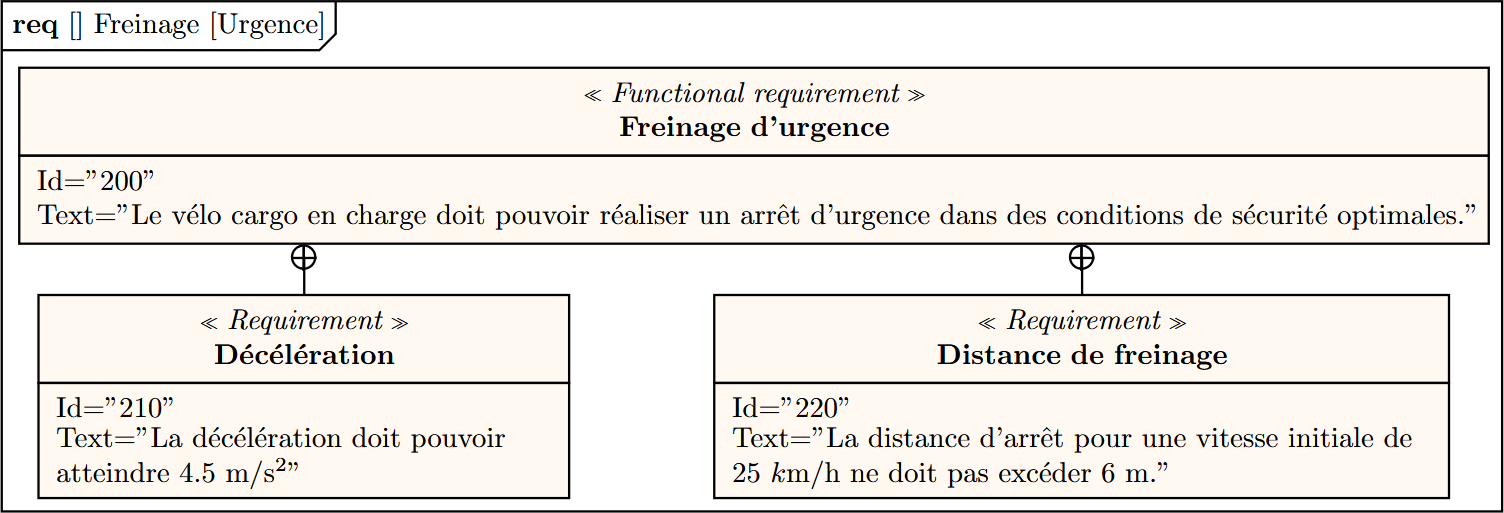
\includegraphics[width=.8\linewidth]{fig_31}
\caption{\label{fig_3_cargo}Extrait du cahier des charges relatif au freinage d'urgence}
\end{figure}



\subsection{Modèle d'étude}
\subsubsection{Définition des ensembles}
On étudie le vélo G4 muni de sa «black box», chargé à son maximum et en mouvement de translation rectiligne dans la direction \(\vec{x}\) (figure \ref{fig_32}). Le cadre est supposé horizontal et la fourche avant est infiniment rigide. Les différents ensembles définis pour l'étude du freinage sont listés dans le tableau \ref{tab_31}. Ces ensembles sont supposés indéformables. Leurs caractéristiques inertielles sont recensées dans le tableau \ref{tab_32}.

Le repère associé au sol (0) est supposé galiléen.

\subsubsection{Modélisation des contacts entre les ensembles}
\paragraph*{Contact roues-sol} 
Les contacts entre les roues et le sol sont modélisés par des liaisons sphère-plan. Le frottement est pris en compte au niveau de ces contacts, la résistance au roulement est négligée, ainsi :

$
\begin{aligned}
& \{0 \rightarrow 1\}=_{I}\left\{\begin{array}{c}
-X_{01} \cdot \vec{x}+Y_{01} \cdot \vec{y} \\
\overrightarrow{0}
\end{array}\right\} \quad \text { où }\left\{\begin{array} { c } 
{ X _ { 0 1 } > 0 } \\
{ Y _ { 0 1 } > 0 }
\end{array} \quad \text { et } \left\{\begin{array}{rl}
\text { si glissement en } I: & X_{01}=f^{\prime} \cdot Y_{01} \\
\text { si non glissement en } I: & X_{01}<f^{\prime} \cdot Y_{01}
\end{array}\right.\right. \\
& \{0 \rightarrow 3\}={ }_{J}\left\{\begin{array}{c}
-X_{03} \cdot \vec{x}+Y_{03} \cdot \vec{y} \\
\overrightarrow{0}
\end{array}\right\} \quad \text { où }\left\{\begin{array} { c } 
{ X _ { 0 3 } > 0 } \\
{ Y _ { 0 3 } > 0 }
\end{array} \quad \text { et } \left\{\begin{array}{rl}
\text { si glissement en } J: & X_{03}=f^{\prime} \cdot Y_{03} \\
\text { si non glissement en } J: & X_{03}<f^{\prime} \cdot Y_{03}
\end{array}\right.\right.
\end{aligned}
$

où \(f^{\prime}\) désigne, selon la configuration, le coefficient de frottement ou d'adhérence du contact roue-sol (supposés égaux). La valeur de \(f^{\prime}\) dépend de nombreux facteurs parmi lesquels l'état du pneumatique et l'humidité de la chaussée (voir tableau \ref{tab_33}).

\paragraph*{Guidages en rotation des roues} Les roues sont en liaison pivot avec l'ensemble (2) :

\begin{itemize}
  \item autour de l'axe \((B, \vec{z})\) pour la roue arrière (1),
  \item autour de l'axe \((C, \vec{z})\) pour la roue avant (3).
\end{itemize}

Ces liaisons sont supposées parfaites.

\paragraph*{Action des freins} Lors du freinage commandé par le cycliste, les freins appliquent sur chaque roue un couple de freinage défini par :
\begin{itemize}
\item pour la roue arrière : \(\overrightarrow{C_{f, 2 \rightarrow 1}}=C_{f 1} \cdot \vec{z}\);
\item pour la roue avant : \(\overrightarrow{C_{f, 2 \rightarrow 3}}=C_{f 3} \cdot \vec{z}\).
\end{itemize}


\begin{table}[!h]
\centering
\begin{tabular}{lll}
\hline
\textbf{Identifiant} & \textbf{Définition} & \textbf{Repère associé} \\
\hline
\((0)\) & Sol & \((O ; \vec{x} ; \vec{y} ; \vec{z})\) \\
\((1)\) & Roue arrière & \(\left(B ; \overrightarrow{x_{1}} ; \overrightarrow{y_{1}} ; \vec{z}\right)\) \\
\((2)\) & Vélo privé de ses roues + pilote + charge & \(\left(G_{2} ; \vec{x} ; \vec{y} ; \vec{z}\right)\) \\
\((3)\) & Roue avant & \(\left(C ; \overrightarrow{x_{3}} ; \overrightarrow{y_{3}} ; \vec{z}\right)\) \\
\hline
\end{tabular}
%Tableau 3.1 - 
\caption{Ensembles définis pour l'étude du freinage \label{tab_31}}
\end{table}




\begin{figure}[!htb]
\begin{center}
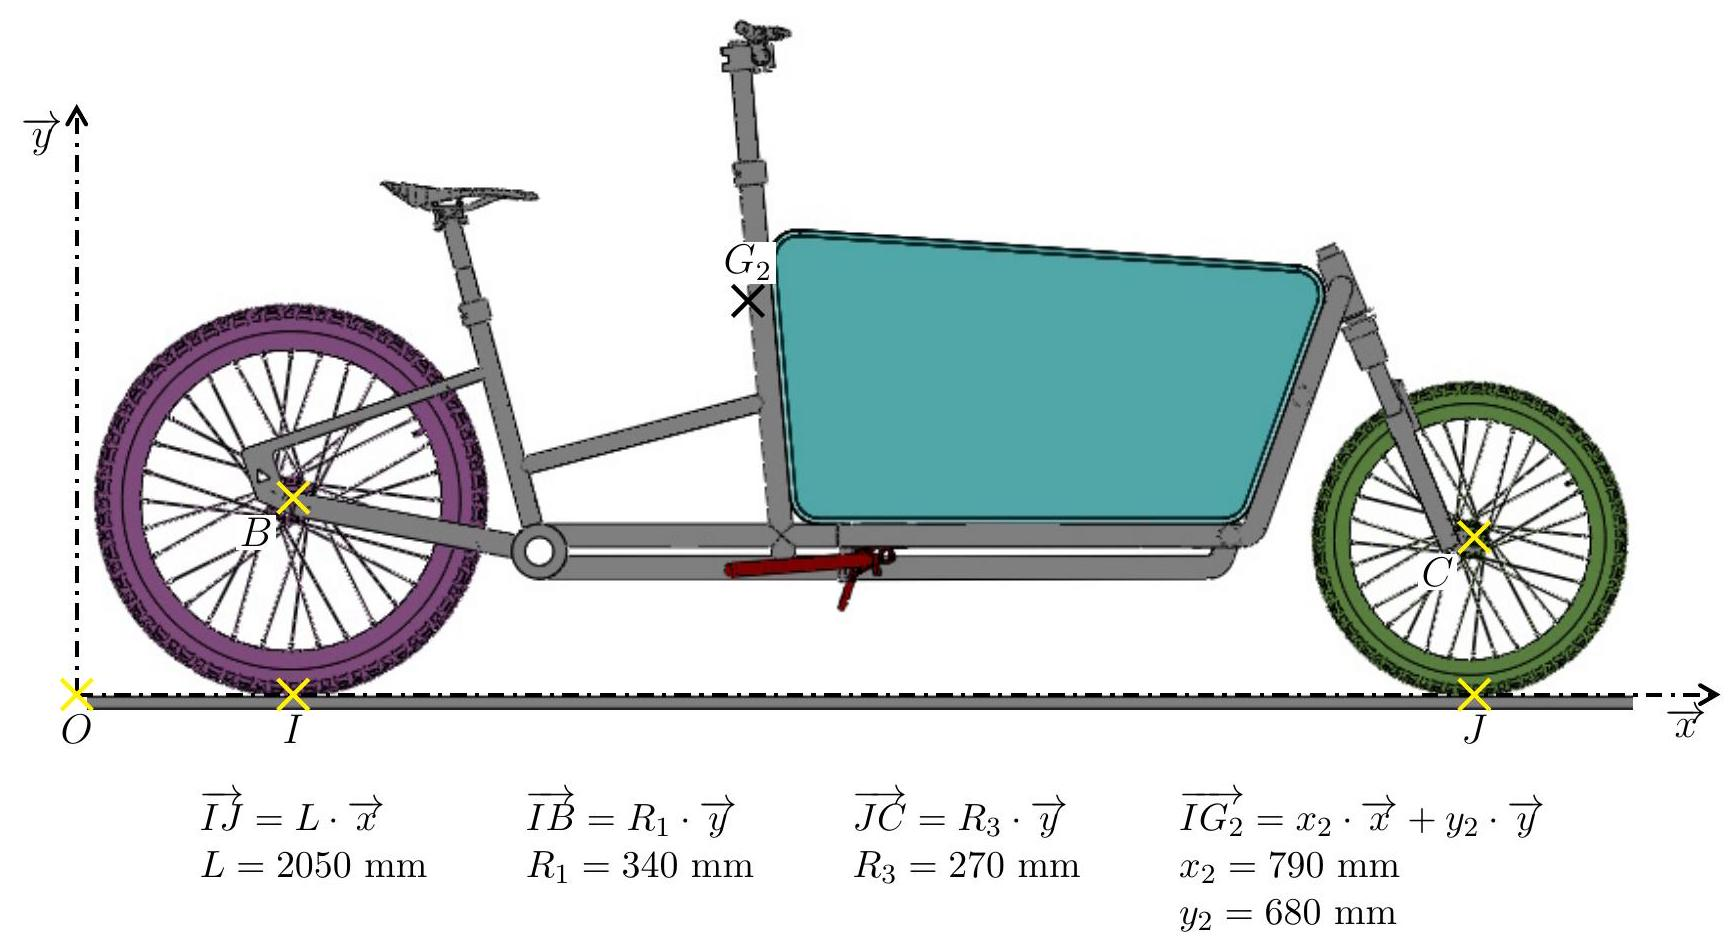
\includegraphics[width=0.8\textwidth]{2024_12_06_8b2ce2e701dae8972925g-08}
% FIG 3.2
\caption{Paramétrage adopté pour le dimensionnement des organes de freinage \label{fig_32}}
\end{center}
\end{figure}


\begin{table}[!h]
\centering
\begin{tabular}{p{4cm}p{3cm}p{3cm}p{4cm}}
\hline
\textbf{Ensemble} & \textbf{Masse} & \textbf{Centre d'inertie}&\textbf{Moment d'inertie au centre d'inertie suivant } $\vect{z}$ \\
\hline
Roue arrière (1) & \(m_{1}=8 \mathrm{~kg}\) & \(B\) & \(I_{B 1}=0.78 \mathrm{~kg} \cdot \mathrm{~m}^{2}\) \\
Ensemble \{Vélo privé de ses roues + pilote + charge \} (2)  & \(m_{2}=245 \mathrm{~kg}\) & \(G_{2}\) & - \\
Roue avant (3) & \(m_{3}=4 \mathrm{~kg}\) & \(C\) & \(I_{C 3}=0.26 \mathrm{~kg} \cdot \mathrm{~m}^{2}\) \\
\hline
\end{tabular}
%Tableau 3.2
\caption{ Caractéristiques inertielles des ensembles pour l'étude du freinage \label{tab_32}}
\end{table}


\begin{table}[!h]
\centering
\begin{tabular}{lll}
 & \textbf{Pneu neuf} & \textbf{Pneu anormalement usé} \\
\hline
Route goudronnée sèche & 0.8 & 0.95 \\
Route goudronnée mouillée & 0.6 & 0.3 \\
\hline
\end{tabular}
%Tableau 3.3 - 
\caption{Valeurs du coefficient de frottement/d'adhérence (supposés égaux) \(f^{\prime}\) en fonction de l'état du pneu et de la route \label{tab_33}}
\end{table}


\subsubsection{Grandeurs cinématiques}
\paragraph*{Vitesses de pivotement des roues} On note \(\omega_{12}\) et \(\omega_{32}\) les vitesses de rotation telles que :
$
\overrightarrow{\Omega(1 / 2)}=\omega_{12} \cdot \vec{z} \quad \text { et } \quad \overrightarrow{\Omega(3 / 2)}=\omega_{32} \cdot \vec{z}
$

\paragraph*{Position, vitesse et accélération du point \(G_{2}\) par rapport au sol}
\begin{itemize}
\item La position selon \(\vec{x}\) du point \(G_{2}\) dans le repère du sol (0) est notée \(x_{G_{2}}: x_{G_{2}}(t)=\overrightarrow{O G_{2}} \cdot \vec{x}\).
  \item La vitesse horizontale de \(G_{2}\) est notée \(v_{G_{2}}: v_{G_{2}}(t)=\dfrac{\mathrm{d} x_{G_{2}}(t)}{\mathrm{d} t}\).
  \item L'accélération horizontale du point \(G_{2}\) est désignée par \(\gamma_{G_{2}}: \gamma_{G_{2}}(t)=\dfrac{\mathrm{d} v_{G_{2}}(t)}{\mathrm{d} t}\).
\end{itemize}

\subsection{Capacité de freinage d'urgence}
\begin{obj}
Déterminer les conditions portant sur les pneumatiques qui permettent d'assurer un freinage d'urgence conforme aux exigences de la figure \label{fig_31}.
\end{obj}

\question{Déterminer l'expression des résultantes dynamiques :}
\vspace{-.25cm}
\textit{
\begin{enumerate}
  \item du solide (1) dans son mouvement par rapport au sol (0) : \(\overrightarrow{R_{d}(1 / 0)}\),
  \item de l'ensemble (2) dans son mouvement par rapport au sol (0) : \(\overrightarrow{R_{d}(2 / 0)}\),
  \item du solide (3) dans son mouvement par rapport au sol (0) : \(\overrightarrow{R_{d}(3 / 0)}\).
\end{enumerate}}
\ifprof
\begin{corrige}-- [UPSTI]
\end{corrige}
\else
\fi

\vspace{.25cm}

\question{ En appliquant le théorème de la résultante dynamique au système matériel \(\{1,2,3\}\), déterminer les expressions :}
\vspace{-.25cm}\textit{
\begin{itemize}
  \item de la somme des composantes tangentielles \(\left(X_{01}+X_{03}\right)\) et
  \item de la somme des composantes normales \(\left(Y_{01}+Y_{03}\right)\)
de l'action du sol sur les roues.
\end{itemize}}
\ifprof
\begin{corrige}-- [UPSTI]
\end{corrige}
\else
\fi

\vspace{.25cm}

On se propose d'équilibrer la répartition du freinage de telle façon que les composantes tangentielles exercées par le sol sur les roues soient identiquement proportionnelles aux composantes normales. On introduit dès lors le coefficient \(k_{f}\) de proportionnalité correspondant tel que :
$
X_{01}=k_{f} \cdot Y_{01} \quad \text { et } \quad X_{03}=k_{f} \cdot Y_{03}
$

\question{Déterminer une expression de \(k_{f}\) en fonction de \(g\) et \(\gamma_{G_{2}}\).}
\ifprof
\begin{corrige}-- [UPSTI]
\end{corrige}
\else
\fi

\question{À partir de l'expression de la condition de non glissement des roues sur le sol, déterminer la valeur limite de \(\gamma_{G_{2}}(t)\) en fonction de \(f^{\prime}\) et \(g\). Montrer alors que toutes les configurations du tableau 3.3 ne permettent pas de satisfaire l'exigence 210.}
\ifprof
\begin{corrige}-- [UPSTI]
\end{corrige}
\else
\fi

On considère à présent uniquement la situation où le freinage peut être réalisé sans glissement. Quels que soient les résultats trouvés précédemment, on définit deux valeurs pour la décélération limite \(\gamma_{\text{lim}}\) :

\begin{itemize}
  \item \(\gamma_{\text {lim }}=-4.5 \mathrm{~m} \cdot \mathrm{~s}^{-2}\) dans le cas du freinage en conditions normales (pneus neufs ou pneus usés sur chaussée sèche),
  \item \(\gamma_{\text {lim }}=-2.95 \mathrm{~m} \cdot \mathrm{~s}^{-2}\) dans le cas du freinage en conditions dégradées (pneus usés sur chaussée mouillée).
\end{itemize}

On suppose de plus que la décélération maximale est immédiatement atteinte lorsque l'utilisateur agit sur les freins. La décélération est supposée constante pendant toute la durée du freinage.


\question{En étudiant le mouvement de l'ensemble \(\{1,2,3\}\) lors du freinage, montrer que la distance de freinage \(d_{f}\) définie par le passage de la vitesse initiale \(v_{0}\) à une vitesse nulle peut s'écrire : \(d_{f}=-\left(v_{0}\right)^{2} /\left(2 \cdot \gamma_{G_{2}}\right)\).}
\ifprof
\begin{corrige}-- [UPSTI]
\end{corrige}
\else
\fi

\question{Conclure quant au respect de l'exigence 220 portant sur la distance de freinage et sur la responsabilité de l'utilisateur.}
\ifprof
\begin{corrige}-- [UPSTI]
\end{corrige}
\else
\fi

\subsection{Dimensionnement des organes de freinage}

\begin{obj}
Valider le dimensionnement des organes de freinage.
\end{obj}

Cette sous-partie vise à établir l'expression du couple que les freins doivent appliquer sur chacune des roues. On établit donc ici une étude de dynamique du mobile lors du freinage en analysant entre autres le mouvement des roues.

\question{Déterminer l'expression du moment dynamique de l'ensemble (2) par rapport au sol (0) au point \(G_{2}: \overrightarrow{\delta\left(G_{2}, 2 / 0\right)}\).}
\ifprof
\begin{corrige}-- [UPSTI]
\end{corrige}
\else
\fi

\question{Déterminer l'expression de la projection sur \(\vec{z}\) :}
\vspace{-.25cm}\textit{
\begin{enumerate}
  \item du moment cinétique au point \(B\) de la roue arrière (1) par rapport au sol \((0): \overrightarrow{\sigma(B, 1 / 0)} \cdot \vec{z}\),
  \item du moment dynamique au point \(B\) de la roue arrière (1) par rapport au sol \((0): \overrightarrow{\delta(B, 1 / 0)} \cdot \vec{z}\).
\end{enumerate}}
\ifprof
\begin{corrige}-- [UPSTI]
\end{corrige}
\else
\fi

\vspace{.25cm}

\question{Déterminer l'expression de la projection sur \(\vec{z}\) du moment dynamique de la roue avant (3) par rapport au sol (0) au point \(C: \overrightarrow{\delta(C, 3 / 0)} \cdot \vec{z}\).}
\ifprof
\begin{corrige}-- [UPSTI]
\end{corrige}
\else
\fi

\question{En supposant qu'il y a roulement sans glissement en \(I\) (respectivement en \(J\)), déterminer la relation entre \(\omega_{12}\) et \(v_{G_{2}}(t)\) (respectivement entre \(\omega_{32}\) et \(v_{G_{2}}(t)\) ).}
\ifprof
\begin{corrige}-- [UPSTI]
\end{corrige}
\else
\fi

\question{En appliquant le théorème du moment dynamique à chacune des roues, montrer que les composantes \(X_{01}\) et \(X_{03}\) ont pour expressions:}
$X_{01}=\dfrac{C_{f 1}+\dfrac{I_{B 1}}{R_{1}} \gamma_{G_{2}}}{R_{1}} \quad \text { et } \quad X_{03}=\dfrac{C_{f 3}+\dfrac{I_{C 3}}{R_{3}} \gamma_{G_{2}}}{R_{3}}
$
\ifprof
\begin{corrige}-- [UPSTI]
\end{corrige}
\else
\fi


\question{En appliquant le théorème du moment dynamique au système matériel \(\{1,2,3\}\) en \(I\), montrer que l'on peut exprimer \(Y_{03}\) sous la forme suivante :}

$
Y_{03}=\dfrac{1}{L}\left[g\left(m_{2} \cdot x_{2}+m_{3} \cdot L\right)-\gamma_{G_{2}}\left(y_{2} \cdot m_{2}+R_{1} \cdot m_{1}+R_{3} \cdot m_{3}\right)+I_{B 1} \cdot \dfrac{\mathrm{~d} \omega_{12}}{\mathrm{~d} t}+I_{C 3} \cdot \dfrac{\mathrm{~d} \omega_{32}}{\mathrm{~d} t}\right]
$
\ifprof
\begin{corrige}-- [UPSTI]
\end{corrige}
\else
\fi


Les relations obtenues lors des questions précédentes amènent aux expressions suivantes :

$
\begin{array}{ll}
X_{01}=\dfrac{R_{1} \cdot C_{f 1}+I_{B 1} \cdot \gamma_{G_{2}}}{R_{1}^{2}} & Y_{01}=\dfrac{1}{L}\left[g\left(m_{2} \cdot\left(L-x_{2}\right)+m_{1} \cdot L\right)+\gamma_{G_{2}}\left(y_{2} \cdot m_{2}+R_{1} \cdot m_{1}+R_{3} \cdot m_{3}+\dfrac{I_{B 1}}{R_{1}}+\dfrac{I_{C 3}}{R_{3}}\right)\right] \\
X_{03}=\dfrac{R_{3} \cdot C_{f 3}+I_{C 3} \cdot \gamma_{G_{2}}}{R_{3}^{2}} & Y_{03}=\dfrac{1}{L}\left[g\left(m_{2} \cdot x_{2}+m_{3} \cdot L\right)-\gamma_{G_{2}}\left(y_{2} \cdot m_{2}+R_{1} \cdot m_{1}+R_{3} \cdot m_{3}+\dfrac{I_{B 1}}{R_{1}}+\dfrac{I_{C 3}}{R_{3}}\right)\right]
\end{array}
$

On suppose de plus que l'on assure une répartition de freinage optimale sous la forme :

$
X_{01}=k_{f} \cdot Y_{01} \quad \text { et } \quad X_{03}=k_{f} \cdot Y_{03}
$

En tenant compte de cette répartition optimale, les relations obtenues précédemment permettent de tracer les évolutions des couples de freinage \(C_{f 1}\) et \(C_{f 3}\) en fonction de la décélération visée (figure 3.3).\\

\begin{figure}[!htb]
\begin{center}
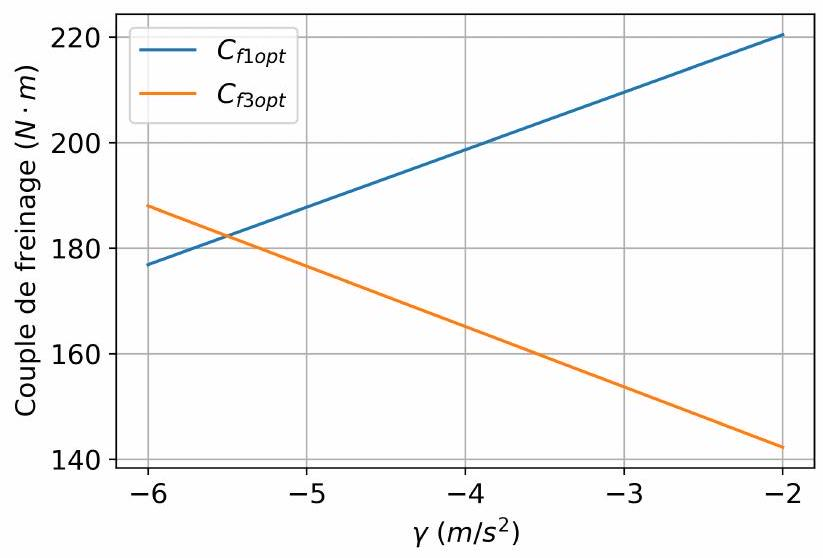
\includegraphics[width=0.6\textwidth]{2024_12_06_8b2ce2e701dae8972925g-11}
\caption{Couples de freinage optimaux en fonction de la décélération visée \label{fig6}}
\end{center}
\end{figure}

\question{Pour une décélération visée «dite d'urgence» conforme à l'exigence 210 de \SI{-4.5}{m.s^{-2}}, déterminer les couples de freinage optimaux à mettre en œuvre sur chacune des roues.}
\ifprof
\begin{corrige}-- [UPSTI]
\end{corrige}
\else
\fi

\question{Conclure quant au système de freins installé sachant que les freins installés sur le G4e permettent d'envisager un couple de freinage maximum de \(250 \mathrm{~N} \cdot \mathrm{~m}\) pour une distance parcourue de \SI{6}{m}.}
\ifprof
\begin{corrige}-- [UPSTI]
\end{corrige}
\else
\fi

Le contrôle du freinage, assuré par le conducteur, est réalisé par l'action de ses mains sur chacune des poignées de frein. Le cycliste module ainsi l'intensité du couple de freinage sur chacune des roues au travers de son ressenti. Les couples de freinage peuvent donc s'en trouver non optimaux.

\question{Proposer une solution technologique de pilotage des freins qu'il serait possible d'intégrer pour optimiser les conditions de freinage.}
\ifprof
\begin{corrige}-- [UPSTI]
\end{corrige}
\else
\fi


